\documentclass [
	a4paper,
	11pt,
	oneside,
	%twoside,
	bibliography=totoc,
	openright,
	numbers=noenddot,
	headings=normal,
	captions=tableheading,
	listof=totoc,
	%chapterprefix,
	headsepline,
	DIV=9,
	BCOR10mm,
	parskip,        
	titlepage,
] {scrbook}


%Begin Dokument

%%
%%Fuer Korrektur eigene Environment fuer Kommentare,etc.
\newenvironment{altertext}{\begin{quote}\small}{\end{quote}}
\usepackage{tikz,ed,fixme} 
\usepackage[framemethod=tikz]{mdframed} \newcommand{\notab}[1]{\textbf{\sffamily\textcolor{blue}{ [[#1]] }}} \mdfdefinestyle{leftbar}{linecolor=blue,linewidth=3pt,topline=false,
rightline=false,bottomline=false}  \mdfdefinestyle{rahmen}{roundcorner=10pt,leftmargin=1, rightmargin=1, linecolor=blue,outerlinewidth=1, innerleftmargin=15, innertopmargin=15,innerbottommargin=15,  skipabove=\topskip,skipbelow=\topskip} \newenvironment{nota}{\begin{quote}\sffamily\hrule}   {\par\smallskip\hrule\end{quote}} 
\newenvironment{VB}{\begin{mdframed}[style=leftbar]\noindent\sffamily\parindent0pt}
{\end{mdframed}\noindent} \newenvironment{VB*}{\begin{quote}\color{blue}}{\end{quote}}  \newcommand{\Del}[2][]{\footnote{Entfernt: \textcolor{brown}{#2} --- #1}} 


%%
%&Anpassung Raender Dokument 
\usepackage{geometry}
%\geometry{a4paper, top=30mm, left=20mm, right=20mm, bottom=30mm,footskip=12mm}
\geometry{a4paper, top=30mm, bottom=30mm,footskip=12mm}

%%%Durchlaufende Nummerierung Fußnoten \footnote
\usepackage{remreset}
\makeatletter
\@removefromreset{footnote}{chapter}
\makeatother
%Fussnote in Table sichtbar
\usepackage{footnote}
\makesavenoteenv{tabular}
\makesavenoteenv{table}
%%%

%%
%% Unterstützung für deutsche Sprache, Umlaute etc.
%%
\usepackage{ngerman}
%\usepackage [ngerman] {babel}
\usepackage [utf8] {inputenc}
\usepackage{csquotes}
\usepackage[T1]{fontenc}
\usepackage{textcomp}

%%Erzeugt für jedes Chapter eine neue Start-Seite
%%mit Nummer des Kapitels in Grau
%\usepackage{longtable}					%js
%\usepackage[grey,helvetica]{quotchap}	%js

%%Zeigt nur die verwendeten Abkuerzungen im Abkuerzungsverzeichnis
\usepackage[printonlyused]{acronym}		%js


%%
%% Diverse Pakete
%%
\definecolor{dunkelrot}{rgb}{102,0,0}
\usepackage{graphicx} 
\usepackage{float}
\usepackage{verbatim}
\usepackage{fancyhdr}
\usepackage{floatflt} 
\usepackage{enumitem}
\usepackage{mathrsfs,amssymb}
\usepackage[intlimits] {empheq}
\usepackage{theorem}
\usepackage{wrapfig}
\usepackage {marvosym}
\usepackage {xcolor}
\usepackage{caption}
\usepackage{subcaption}
\usepackage{scrhack}
\usepackage{microtype}
\usepackage{setspace}
\usepackage{array, tabularx}
\usepackage{amsmath}
\usepackage{booktabs}
\usepackage{ragged2e}
\usepackage{multirow}
\usepackage[left]{eurosym}	
\usepackage[section]{placeins}			%js
\usepackage{epigraph}					%js
\setlength{\epigraphwidth}{0.4\textwidth}
\usepackage{framed}

%%
%% Anpassung an Aussehen bei Click auf Links und Verlinkungen des Inhaltsverzeichnis
\usepackage[hyphens]{url}

\usepackage[colorlinks,pdfpagelabels,pdfstartview = FitH,bookmarksopen = true,bookmarksnumbered = true,linkcolor = black,plainpages = false,hypertexnames = false,citecolor = black, urlcolor=black] {hyperref}

%%use the same style for url as in the document
\urlstyle{same}
%%

%%
% Anpassung der Ueberschriften
\usepackage{titlesec}
\titlespacing{\chapter}{0pt}{-6em}{6pt}
\titlespacing{\section}{0pt}{6pt}{6pt}
\usepackage{listingsutf8}

%%
% Anpassung Zeilenabstand
\linespread {1.5}


%%
%% Verhindert überhängende Absatzteile
%%
\clubpenalty10000
\widowpenalty10000
\displaywidowpenalty=10000

%%Anpassung schreiben auf 2. Seite nach chapter
\renewcommand*\chapterheadstartvskip{\vspace*{-0.5cm}}
%%
\setlength{\parindent}{0pt}
\setlength{\parskip}{1.4ex plus 0.35ex minus 0.3ex}

% Schrift ----------------------------------------------------------------------
\usepackage{lmodern} % bessere Fonts
%\usepackage{relsize} % Schriftgröße relativ festlegen
\usepackage{microtype} % AL: Verbessert den Schriftsatz

%%
%% Schriftarten
%%
\renewcommand{\sfdefault}{phv}
\renewcommand{\ttdefault}{ppl}
\renewcommand{\rmdefault}{phv}
%\KOMAoptions{DIV=last}
% change Font during text
\newcommand{\changefont}[3]{
\fontfamily{#1}\fontseries{#2}\fontshape{#3}\selectfont}


%%
%% Formatierung des Literaturverzeichnisses
%%
%\bibliographystyle{plaindin} % Nummern und alphabetisch sortiert
\bibliographystyle{alphadin} % Buchstaben und sortiert
%\bibliographystyle{abbrvdin} % Nummern und abgekürzte Namen
%\bibliographystyle{unsrtdin} % Nummern und unsortiert

% fortlaufendes Durchnummerieren der Fussnoten ----------------------------------
\usepackage{chngcntr}

%%
%% Trennungsregeln
%%
\hyphenation{Sil-ben-trenn-ung}

%%
%% Seitenlayout
%%
\pagestyle{fancy}

\setcounter{tocdepth}{3}	% tiefe des inhaltsverzeichnisses
\setcounter{secnumdepth}{3} % Nummerierung der Überschriftentiefe festlegen


%%
%% Schönere Bullets bei Aufzählungen
%%
\renewcommand{\labelitemi}{$\bullet$}
\renewcommand{\labelitemii}{$\circ$}
\renewcommand{\labelitemiii}{$\cdot$}

%%
%% Set Path fuer Bilder
\graphicspath{{img/}}

%js definition-umgebung setzen!
\newtheorem{definition}{Definition}
% js end definition

%%
%%Quellcode Formatierungen Java
%%
\definecolor{javared}{rgb}{0.6,0,0} % for strings

\lstdefinestyle{javacode}{
	language=Java, 
   	basicstyle=\footnotesize, 
    	frame=lines,
   	keywordstyle=\bf{\color{blue!80!black!100}}, 
   	identifierstyle=, 
   	xleftmargin=15pt,
    	framexleftmargin=15pt,
    	tabsize=3,
   	frame=shadowbox,
    	rulesepcolor=\color{gray}, 
   	commentstyle=\color{green!50!black!100}, 
   	numberblanklines=false,
   	stringstyle=\color{javared}, 
   	breaklines=true, 
   	numbers=left, 
   	numberstyle=\tiny,
     numbersep=5pt,
    	breaklines=true,
    	showstringspaces=false,
}
%%
%%Quellcode Formatierung Android XML
\definecolor{darkgreen}{rgb}{0,0.5,0}
\lstdefinestyle{xmlcode}{
    language=xml,
    sensitive=true,
    tabsize=3,
    frame=lines,
    frame=shadowbox,
    rulesepcolor=\color{gray},
    xleftmargin=20pt,
    framexleftmargin=15pt,
    keywordstyle=\color{magenta}\bf,
    commentstyle=\color{darkgreen},
    stringstyle=\color{javared},
    numbers=left,
    numberstyle=\tiny,
    numbersep=5pt,
    breaklines=true,
    showstringspaces=false,
    basicstyle=\footnotesize,
    morecomment=[s]{<?}{?>},
    morecomment=[s]{<!-}{-->},
    alsoletter={<>=-}, 
    moredelim=[s][\color{black}]{>}{<},
    tag=[s],
    identifierstyle=\bf{\color{blue!80!black!100}},
    alsodigit={:},
}

%%
%%Quellcode Formatierung HTML
\lstdefinestyle{html5}{
    language=html,
    sensitive=true,
    tabsize=3,
    frame=lines,
    frame=shadowbox,
    rulesepcolor=\color{gray},
    xleftmargin=20pt,
    framexleftmargin=15pt,
    keywordstyle=\bf{\color{blue!80!black!100}},
    commentstyle=\color{darkgreen},
    stringstyle=\color{javared},
    numbers=left,
    numberstyle=\tiny,
    numbersep=5pt,
    breaklines=true,
    showstringspaces=false,
    basicstyle=\footnotesize,
    morecomment=[s]{<!-}{-->},
    alsoletter={<>=-}, 
    moredelim=[s][\color{black}]{>}{<},
    tag=[s],
    emphstyle={\color{magenta}},
    identifierstyle=\bf{\color{blue!80!black!100}}
}


%%
%% hier Namen etc. einsetzen
%%
\newcommand{\nameone}{Sara Steisslinger}
\newcommand{\matnrone}{Matrikelnummer: 823825}
\newcommand{\stdrichtungone}{WiWi BSc}
\newcommand{\stdrichtungtwo}{WiWi MSc}

\newcommand{\nametwo}{Jasmin Klose}
\newcommand{\matnrtwo}{Matrikelnummer: 757415}
\newcommand{\namethree}{Manuel Buchert}
\newcommand{\matnrthree}{Matrikelnummer: 758373}
\newcommand{\namefour}{Florian Rotter}
\newcommand{\matnrfour}{Matrikelnummer: 761110}
\newcommand{\namefive}{Daniel Glunz}
\newcommand{\matnrfive}{Matrikelnummer: 702033}
\newcommand{\namesix}{Manuel Ott}
\newcommand{\matnrsix}{Matrikelnummer: 770969}


\newcommand{\titel}{Dokumenten- /Konfigurationsmanagement in verteilten Software-Projekten}
\newcommand{\semester}{Sommersemester 2014}
\newcommand{\gutachter}{Prof.\ Dr.\ Franz Schweiggert}
\newcommand{\fakultaet}{Fakultät für Mathematik und Wirtschaftswissenschaften}
\newcommand{\institut}{Institut für angewandte Informationsverarbeitung}
\newcommand{\arbeit}{Begleit-Seminar zur Vorlesung\\Entwicklung und Betrieb von Informationssystemen}

%%
%% Setzt Autor und Titel in den Metadaten des erzeugten Dokumentes
%%
\pdfinfo{
    /Author (\nameone \nametwo \namethree \namefour \namefive)
    /Title (\titel)
    /Producer (pdfeTex 3.14159-1.30.6-2.2)
    /Keywords ()
}
\hypersetup{
    pdftitle=\titel,
    pdfauthor=\nameone \nametwo \namethree \namefour \namefive
    pdfsubject={\arbeit},
    pdfproducer={pdfeTex 3.14159-1.30.6-2.2},
    colorlinks=false,
    pdfborder=0 0 0
}


\begin {document}

\frontmatter
\begin{titlepage}

	\begin{figure} [!h]
		\begin{flushright}
			
\includegraphics[scale=0.125]{img/Unilogo.jpg}
		\end{flushright}
	\end{figure}

	\begin{center}
		\vspace{-0.8cm}
		{\Large\bfseries Universit"at Ulm\\
			\fakultaet\\
			\institut\\
			\arbeit\\
			\semester\\
		} 
	\end{center}
	\vspace{-0.3cm}
	{\large
		Titel der Ausarbeitung:
		\begin{center}
			\vspace{-0.4cm}
			\textbf{\titel}
		\end{center}
	}

	\begin{center}

			\vspace{-0.8cm}
\begin{tabular} {p{4cm}  p{5cm} p{5cm}}

\textbf{\nameone} &\matnrone & Studienrichtung: \stdrichtungone \\
	\textbf{\nametwo} &\matnrtwo & Studienrichtung: \stdrichtungone \\
	\textbf{\namethree}& \matnrthree & Studienrichtung: \stdrichtungone\\
	\textbf{\namefour} & \matnrfour & Studienrichtung: \stdrichtungone\\
	\textbf{\namefive} & \matnrfive & Studienrichtung: \stdrichtungtwo\\ 
	\textbf{\namesix} & \matnrsix & Studienrichtung: \stdrichtungone
\end{tabular}

	\end{center}
	\begin{framed}
			\vspace*{-0.3cm}

			%%
%% Versicherung
%%

\minisec{Ehrenw"ortliche Erklärung}

Wir versichern, dass wir die Seminararbeit gemeinsam verfasst, andere als die angegebenen Quellen und Hilfsmittel nicht benutzt und uns auch sonst keiner unerlaubten Hilfe bedient haben. 
\vspace{3cm}

Ulm, den \hspace{0.2cm} \line(1,0){90} \hspace{3cm} \hrulefill

\hfill {\footnotesize Unterschriften}
\vfill


		\end{framed}


		
	\end{titlepage}

	%\newpage\thispagestyle{empty}


%%Anpassung der Kopf- und Fusszeilen auf den einzelnen Seiten

\fancypagestyle{plain}{
\fancyhf{}
\fancyhead[L] {\small \sffamily \leftmark}%
\fancyfoot[R] {\small \sffamily  \thepage}
}

\pagestyle{fancy}
\fancyhf{}
\fancyhead[L] {\small \sffamily \leftmark}%
\fancyfoot[R] {\small \sffamily  \thepage}
\renewcommand{\chaptermark}[1]{%
\markboth{\thechapter. #1}{}
\renewcommand{\sectionmark}[1]
{\markright{\small\sf\thesection\ ##1}}%	
}	



%Einbinden des Abkuerzungsverzeichnisses
\tableofcontents %Inhaltsverzeichnis

%\listoftables % Tabellenverzeichnis 


%Hahupdokument
\mainmatter

\chapter {Einleitung}

\section {Motivation}
Mit immer fortschreitender Globalisierung entwickelt sich auch die Struktur der Unternehmen weiter. Viele Unternehmen entwickeln sich hin zu multinationalen Konzernen. Hierbei müssen sich alle Bereiche den neuen Anforderungen anpassen. Dies betrifft auch die Softwareentwicklung innerhalb der Unternehmen. Um eine konzernweit einsetzbare Software zu entwickeln, setzten Unternehmen immer mehr auf eine Kooperation von Entwicklungsteams. Der gesamte Software-Entwicklungsprozess wird zerlegt und von verschiedenen Mitarbeitern oder Teams vollzogen. Was früher noch in einer Abteilung geschah, Passiert heute um den ganzen Globus verteilt. So ist es bei vielen Unternehmen Realität, dass ein Teil der Software aus Deutschland, ein anderer aus China und der dritte Teil aus Indien stammt. Hierbei kommt es schnell zu neuen Problemen, die durch die Zergliederung auftreten. Kommunikation wird als wichtige Voraussetzung zur Verwaltung der Ressource „Wissen“ angesehen. „Softwareentwicklung ist von Natur aus teambasiert“ \cite{einleitung}. In verteilten Projekten kommt der Kommunikation eine noch größere Bedeutung zu. Es muss Wissensaustausch über Landes- oder sogar Kontinentgrenzen hinweg betrieben werden, was oft eine schwere Aufgabe darstellt. So hat \acs{z. B.} eine Studie aufgezeigt, dass persönliche Treffen nicht durch Kommunikationsmedien ersetzt werden können. Trotz Videokonferenzen und  Life-Chats, ist die Face-to-Face Kommunikation durch Reisen unabdingbar. Durch die verteilte Arbeit mehrerer Personen, rückt aber auch die Verwaltung der Versionen von Programmen und Dokumenten in den Vordergrund. Es müssen Regeln definiert werden, wer etwas ändern kann, wann dies geschehen darf oder in welcher Reihenfolge. 
\section{Gliederung}
Diese Arbeit greift zuerst das Thema Software Configuration Management auf und behandelt seine einzelnen Aspekte.
Zuerst wird die Konfigurationsidentifikation behandelt, anschließend folgt das Build Management, das Versionsmanagement, ebenso wie das Release und schließlich das Change Management.

%nur  beispielhaft zur visualisierung drinnen:
%\include{chapters/inmemory}
%nur  beispielhaft zur visualisierung drinnen:
%\include{chapters/sap}

\chapter{Software Configuration Management (\acs{SCM})}
Steuert und verwaltet verteilte Software-Projekte.
Ganz normaler Text.




%einbauen? nicht zu umfangreich?
%\chapter{Verlinkung}
\section{Vertical Slice}
Hier geht es um die Auftrennung von User-Stories in zeitliche Abschnitte, wie man es überlicherweise auch in Scrum vorfindet.

\section{Horizontal Slice}



%einbauen? nicht zu umfangreich?
%\chapter{Synchronisation}



%ab hier SCM:
\chapter{Konfigurationsidentifikation}
\section{Konfigurationsidentifikation / Requirements}
Am Anfang eines jeden Software-Projektes sollte die zielgerichtete Festsetzung von Anforderungen (engl.: Requirements) stehen. Auch wenn dieser Aspekt viel zu häufig bedeutend geringer behandelt wird, als es eigentlich notwendig wäre, hat sich daraus inzwischen eine eigene wissenschaftliche Teildisziplin entwickelt. Betrachtet man große Projekte, die über einen langen Zeitraum entwickelt werden, ist eine Orientierung anhand der ursprünglichen Anforderungen von höchster Priorität, da sonst oftmals die Gefahr besteht, den eigentlichen Zweck der Software aus dem Fokus zu verlieren. Außerdem muss man passend auf Anpassungen in den Anforderungen reagieren können. Durch Arbeitsteilung und der daraus resultierenden Spezialisierung innerhalb von Projektgruppen, kann es schnell zu Verständnisproblemen und Kommunikationsschwierigkeiten kommen, die wiederum eine unpassende Problembehandlung nach sich ziehen können. Es ist somit zwingend erforderlich, gleich zu Anfang der Software-Entwicklung die entsprechenden Konfigurationsaspekte zu identifizieren und diese zwischen den beteiligten Personen zu synchronisieren, damit sich während der Arbeitsprozesse keine Eigenschaften aus einem Selbstzweck entwickeln, die den eigentlichen Vorgaben nicht dienlich sind.
%
%\section{Beteiligte Personen}
%Es liegt auf der Hand, dass verteilte Softwareprojekte zumeist ein hohes Maß an Arbeitsteilung aufweisen. Dabei agieren die beteiligten Personen häufig auch räumlich voneinander getrennt. Ferner muss man hinsichtlich der Anforderungen außerdem noch zwischen verschiedenen Interessensgruppen differenzieren, welche im Regelfall auch unterschiedliche Sichtweisen und Erwartungen bezüglich des Projektes haben. Im Allgemeinen muss man zwischen Stakeholdern und der Projektumgebung, bzw. den Projektverantwortlichen unterscheiden. Wie bereits erwähnt ist die korrekte Handhabe von Anforderungen wichtig, um den ursprünglichen Projektzweck nicht zu verfehlen. Man sollte die beteiligten Personenkreise aber auch hinsichtlich der Rückverfolgbarkeit (traceability) von Anforderungen separat betrachten.
%\\
%\textbf{Stakeholder (Auftraggeber)}
%\\
%Als Stakeholder werden in diesem Kontext alle Interessensgruppen gesehen, welche die Kundensicht auf das Projekt repräsentieren. Sie stellen also vor allem Anforderungen aus der Benutzersicht auf, die weniger explizit und auf das Endergebnis gerichtet sind. Diese Anforderungen sind von höchster Relevanz und geben die Rahmenbedingungen für detailliertere Konfigurationsaspekte vor. 
%\\
%\textbf{Projektumgebung (Auftragnehmer)}
%\\
%In erster Linie sind sie für die Realisierung der gestellten Anforderungen zuständig und befassen sich mit der Umsetzung des kompletten Software-Projekts. Aber es ist naheliegend, dass sich während dieses Prozesses auch hieraus neue Anforderungen ergeben, ohne die das Projekt nicht möglich ist. Diese Anforderungen sind wesentlich näher an die eigentliche Softwareentwicklung angelehnt und entstehen oft viel später als die Konfigurationsaspekte der Shareholder.

\section{Requirements Engineering / Requirements Management}
Wird hinsichtlich der Anforderungen bereits sauber gearbeitet, verringern sich Fehlerursachen und ein mögliches Scheitern des Software-Projekts erheblich. Wichtig ist hierbei vor allem zu verstehen, dass zunächst nur die Identifizierung und Handhabe von reinen Anforderungen relevant ist und noch keinerlei Bezug auf eine mögliche Umsetzung genommen werden sollte. Somit zeichnen sich gute Anforderungen durch einige Qualitätskriterien aus, die als grundlegende Voraussetzungen für ihre Verwertbarkeit angesehen werden können. 
\\
Qualitätskriterien einzelner Anforderungen:
\\
\begin{itemize}
	\item Eindeutig
	\item Korrekt (besser: „adäquat“ oder „valide“)
	\item Klassifizierbar (bezüglich juristischer Verbindlichkeit)
	\item Konsistent (in sich und mit externen Vorgaben)
	\item Testbar (Erfüllung nachprüfbar)
	\item Aktuell gültig
	\item Verstehbar (für alle Stakeholder)
	\item Realisierbar
	\item Notwendig
	\item Bewertbar (hinsichtlich Wichtigkeit, Kritikalität oder Priorität)
\end{itemize}

\cite{partsch-re}

\section{Funktionale Anforderungen}
Funktionale Anforderungen legen ausschließlich fest, was das System tun soll (funktional). Es wird jedoch nicht spezifiert, wie die Umsetzung zu erfolgen hat oder welche Eigenschaften damit verbunden sind. Typische funktionale Anforderungen sind:
\begin{itemize}
	\item Eingaben und deren Einschränkungen (Daten, Ereignisse, Stimuli, ...)
	\item Bereitgestellte Dienste („Funktionen“), die das System ausführen können soll
	\subitem Umformung von Daten („funktionales Verhalten“)
	\subitem Verhaltensweisen, abhängig von Ereignissen/Stimuli („reaktives Verhalten“)
	\item Ausgabe (Daten, Fehlermeldungen, Reaktionen, ...)
	\item 	Manchmal auch
	\subitem Relevante Systemzustände („Betriebsmodi“)
	\subitem Zeitliches Verhalten des Systems
\end{itemize}

\cite{partsch-re}

\section{Nicht-funktionale Anforderungen}
Anders als funktionale Anforderungen, beschreiben die nicht-funktionalen Anforderungen, wie gut ein System etwas tun soll (qualitativ). Abhängig des zu entwickelnden Systems können diese Anforderungen von unterschiedlichster Art sein. In diesem Zusammenhang werden über den ISO Standard 9126 hauptsächlich folgende sogenannte Qualitätsattribute für nicht-funktionale Anforderungen beschrieben, die für die meisten Projekte zutreffen:

\begin{itemize}
	\item Performanz
	\item Funktionalität
	\item Usability
	\item Portabilität
	\item Sicherheit
\end{itemize}

\cite{fraunhofer}

\section{Dokumentation (Anforderungsspezifikation)}
Von entscheidender Relevanz für einen strukturierten und zielgerichteten Entwicklungsprozess ist eine angemessene Dokumentation der Anforderungen. Dadurch bleiben die wesentlichen Konfigurationsdetails im Blickfeld und es wird vermieden, dass sich Aspekte in die Systementwicklung einschleichen, die mit den ursprünglichen Anforderungen in keinem Zusammenhang stehen. 
Es hat sich als förderlich erwiesen, eine separate Dokumentation der Anforderungen von Kunden und Entwicklern umzusetzen, damit die ursprünglichen Konfigurationsdetails nicht durch die Konzepte der technischen Umsetzung verfälscht werden und alle beteiligten Parteien über Dokumente verfügen, 
die ihre fachlichen Konventionen und deren Rolle innerhalb des Projekts adäquat abbilden. Als Resultat entstehen 
verschiedene Anforderungsdokumente, die dann als Basis für die Entwicklung dienen und zumeist auch die Grundlage der Kommunikation zwischen Stakeholdern bilden. Die wichtigsten Anforderungsdokumente, das Lasten- und 
Pflichtenheft, werden in den folgenden Kapiteln nochmals detailliert beschrieben. 
Im weiteren Fortgang des Projekts werden die Anforderungen aus diesen Dokumenten dann oft über spezielle Anforderungsmanagement-Software verwaltet und umgesetzt. Dadurch lassen sich Interdependenzen zwischen verschiedenen Teilsystemen einfacher abbilden und zurückverfolgen und man hat eine einheitliche Datenbasis für alle Beteiligten. Ferner lassen sich hierdurch außerdem Änderungen an den Konfigurationen einfacher pflegen und in das komplette System einfügen, ohne Fehler zu provozieren, die durch die komplexen Zusammenhänge innerhalb der Anforderungen leicht entstehen können, wenn nachträgliche Anpassungen erfolgen.
\cite{fraunhofer-anforderung}

\section{Lastenheft}
Das Lastenheft beschreibt den Soll-Zustand der zu entwickelnden Software und enthält alle ermittelten und an das System verbindlich gestellten Anforderungen. Auch hier unterscheidet man zwischen funktionalen und nicht-funktionalen Anforderungen, die auch als solche gekennzeichnet sind. 
Es dient oft auch als Grundlage für Ausschreibungen bei der Projektvergabe und ist fester Vertragsbestandteil zwischen Auftraggeber und Auftragnehmer. Die darin enthaltenen Spezifikationen legen die Rahmenbedingungen bezüglich der Entwicklung beim Auftragnehmer fest und werden von diesem dann in das Pflichtenheft überführt. Auf Grundlage des Lastenhefts wird also die gesamte Entwicklung des geforderten Systems begründet.
Analog zur Konfigurationsidentifikation enthält dieses Dokument noch keine Aspekte bezüglich der expliziten Entwicklung und Umsetzung des Software-Projekts, sondern lediglich Anforderungen an das spätere \Gu Enderzeugnis\Go. 
Das Lastenheft sollte möglichst so gestaltet sein, dass Veränderungen an den Spezifikationen nachträglich ergänzt und verändert werden können und eine Rückverfolgung (traceability) dieser Prozesse möglich ist. Denn zumeist wird es vor Projektbeginn und auch während der Entwicklung an Veränderungen in den Anforderungen angepasst. Der Grund hierfür ist einerseits die Synchronisation der Anforderungen zwischen Stakeholdern und Auftragnehmern vor Projektbeginn und andererseits die Berücksichtigung von Aspekten, die erst in der tatsächlichen Entwicklungsphase auftreten.
\cite{brd-lastenheft}

\section{Pflichtenheft}
Das Pendant zum Lastenheft stellt das Pflichtenheft dar. 
In diesem Dokument werden die Gesamtspezifikationen des Projekts seitens des Auftragnehmers konkretisiert und hinsichtlich der tatsächlichen technischen Umsetzung festgelegt. Anhand der Anforderungen des Lastenhefts wird in diesem Rahmen eine erste Grobarchitektur des Systems entwickelt und geeignet beschrieben. Ebenfalls werden neben der Entwicklung des eigentlichen Systems auch zu entwickelnde 
Untersysteme identifiziert und den jeweiligen Anforderungen zugeordnet, was auch eine erste Arbeitsteilung zwischen den Entwicklern nach sich zieht. Darüber hinaus werden auch vertragliche Aspekte einbezogen, die den Lieferumfang des fertigen Gesamtsystems und die damit verbundenen Abnahmekriterien umfassen. Um sicher zu stellen, dass letztlich alle Anforderungen im Pflichtenheft berücksichtigt und für eine konkrete Umsetzung eingeplant sind
, wird eine Anforderungsverfolgung, sowohl bezüglich des Lastenhefts als auch in Richtung des Systems und den entsprechenden Untersystemen durchgeführt. Die Ausarbeitung des Pflichtenhefts erfolgt innerhalb der Projektumgebung beim Auftragnehmer zwischen den Experten, die für die spätere Erstellung der Systemkomponenten (evtl. auch Untersysteme) zuständig sind
, sowie den Projektverantwortlichen, die ein Hauptaugenmerk auf den Gesamtentwurf des Systems haben und diesbezüglich auch in engem Kontakt mit dem Auftraggeber stehen. Dieser wiederum prüft, ob die Gesamtspezifikationen des Pflichtenhefts seinen Vorgaben entsprechen. Beide Dokumente entstehen somit in sehr 
enger Synchronisation zwischen allen Beteiligten des Projekts und unterliegen während des Entwicklungsprozesses auch dem Anpassungsprozess von Anforderungen und Umsetzungsentwürfen, was eine Veränderlichkeit und Nachverfolgbarkeit beider Dokumente voraussetzt.

\cite{brd-lastenheft}


\chapter{Build Management/ System Building}

Hat man nun den Quellcode der einzelnen Software Komponenten in dem Software- Projekt erstellt, dann möchte man diesen ausführbar machen. Hierum kümmert sich der Build Prozess. Dieser Prozess ist zuständig für das Kompilieren und Linking der einzelnen Software Komponenten in ein ausführbares System. Da die Abhängigkeiten von den Quellcodes, Bildern und weiteren Artefakten bei großen Projekten sehr komplex und unübersichtlich sind, empfiehlt es sich, diese Abhängigkeiten nicht alle manuell zu kompilieren. Hinzu kann natürlich noch kommen, dass für unterschiedliche Systeme unterschiedliche Kombinationsmöglichkeiten von Einzelkomponenten für den Build Prozess benötigt werden. Man erkennt also, dass das einfache kompilieren von Quellcode für ein Software Projekt nicht ausreicht, sondern man weitreichende Überlegungen dazu anstellen muss.
\\
Für diesen Build Schritt in der Softwareentwicklung gibt es inzwischen Unterstützung von automatischen Tools. 
Diese Tools enthalten meistens eine Abhängigkeitsspezifikationssprache und einen Interpreter für  diese Sprache. Ebenso ist meist noch die Möglichkeit zur verteilten Kompilation, die Auswahl von Tools und Support für die Instanziierung des Softwareprojektes gegeben. 
\\
Das bekannteste Tool für UNIX ist make für die C/C++ Entwicklung. Make ist dafür zuständig die Abhängigkeiten zwischen Sourcecode und Objektcode zu beobachten und re-kompiliert automatisch die Sourcen welche nach dem Erstellungsdatum des zugehörigen Objektcodes verändert wurden. Die Abhängigkeiten werden in Makefiles abgebildet, wie auch im folgenden Code ersichtlich wird:

\lstinputlisting[style=makefile,label=makefile,caption=Makefile für Speicherverwaltung aus Systemnahe Software 1-WS 2013/14]{code/Makefile}

In Listing \ref{makefile} werden zuerst die Quellen, die Objekte( die Abhängigkeiten) und die Zielquelle definiert, ebenso der benötigte Kompiler mit Option.
Anschließend werden die einzelnen Befehle beschrieben, also was passiert bei dem Aufruf von \textit{make clean, make realclean} und \textit{make depend}. In den Zeilen 15-17 findet man dann die einzelnen Abhängigkeiten, die mit make depend gefunden wurden.
\\
Weitere bekannte Tools sind Apache Ant, das wohl häufigste verwendete Tool für Java, das analog zu make in einer Datei build.xml die Abhängigkeiten beschreibt, Maven (ebenfalls Java), Jam, MS Build (.NET) und scons.
Doch auch an solche automatischen Tools gibt es eine Anforderungsliste. 
\cite{bib:se}
\begin{itemize}
\item Enthalten die Build Anweisungen alle benötigten Komponenten ?
\item Ist für jede Einzelkomponenten die richtige Version spezifiert?
\item Sind alle benötigten Dateien verfügbar ?
\item Sind die Referenzen innerhalb der Komponenten richtig, also ruft die eine Komponente eine andere mit den richtigen Parametern und Namen auf?
\item Wird die Software auch für das richtige Betriebssystem erstellt?
\item Mit welcher Kompilerversion und weiteren benötigten Software-Tools wird dieser Build-Prozess durchgeführt? 	
\end{itemize}

\subsection{Continous Build}
Schnell stellt sich jedoch die Frage wie oft denn ein solcher Build Prozess durchgeführt werden soll? Soll er nach jeder Änderung, jeder fertigen Teilkomponente durchgeführt werden, um die Funktionen zu testen, oder soll erst am Ende vom Projekt ein kompletter Durchlauf des Build-Prozesses durchlaufen?
\\
Hierfür gibt es keine richtige und falsche Antwort. Die sollte je nach Komplexität des Softwareprojekt individuell entschieden werden. Denn ein solcher Build Prozess kann je nach Komplexität der zu erstellenden Software sehr rechenintensiv und lange sein. 
\\
Zum einen wird ein Build aufwendiger, je seltener dieser durchgeführt wird, da die Fehlerwahrscheinlichkeit steigt und die Einzelkomponenten der Software auseinander laufen können.
\\
Anderseits wiederum ist das ein Nachteil wenn man den Build zu oft durchführt, da bei großen Software Projekten viele Ressourcen benutzt werden, die der Build zu berücksichtigen hat und somit immer rechenintensiver wird.
\\
Die optimale Strategie muss für jedes Softwareprojekt individuell gefunden werden.
Wenn man nach jeder Änderung ein Build durchführen möchte, 
dann bezeichnet man dies als Continuous Integration.
Durch Verwendung von Tools kann hierbei eine Überwachung der Ressourcen und der Aufruf des Build-Tools automatisiert werden. Ebenso kann die Automatisierung des Test nach dem erfolgten Build erfolgen. \cite{build-seminar}, \cite{software-analysis}
\\
Im der folgenden Abbildung \ref{fig:ci} sieht man die Abhängigkeiten, die in einem Software-Projekt vorliegen, darunter auch den Build Prozess.

\begin{figure}[H]
	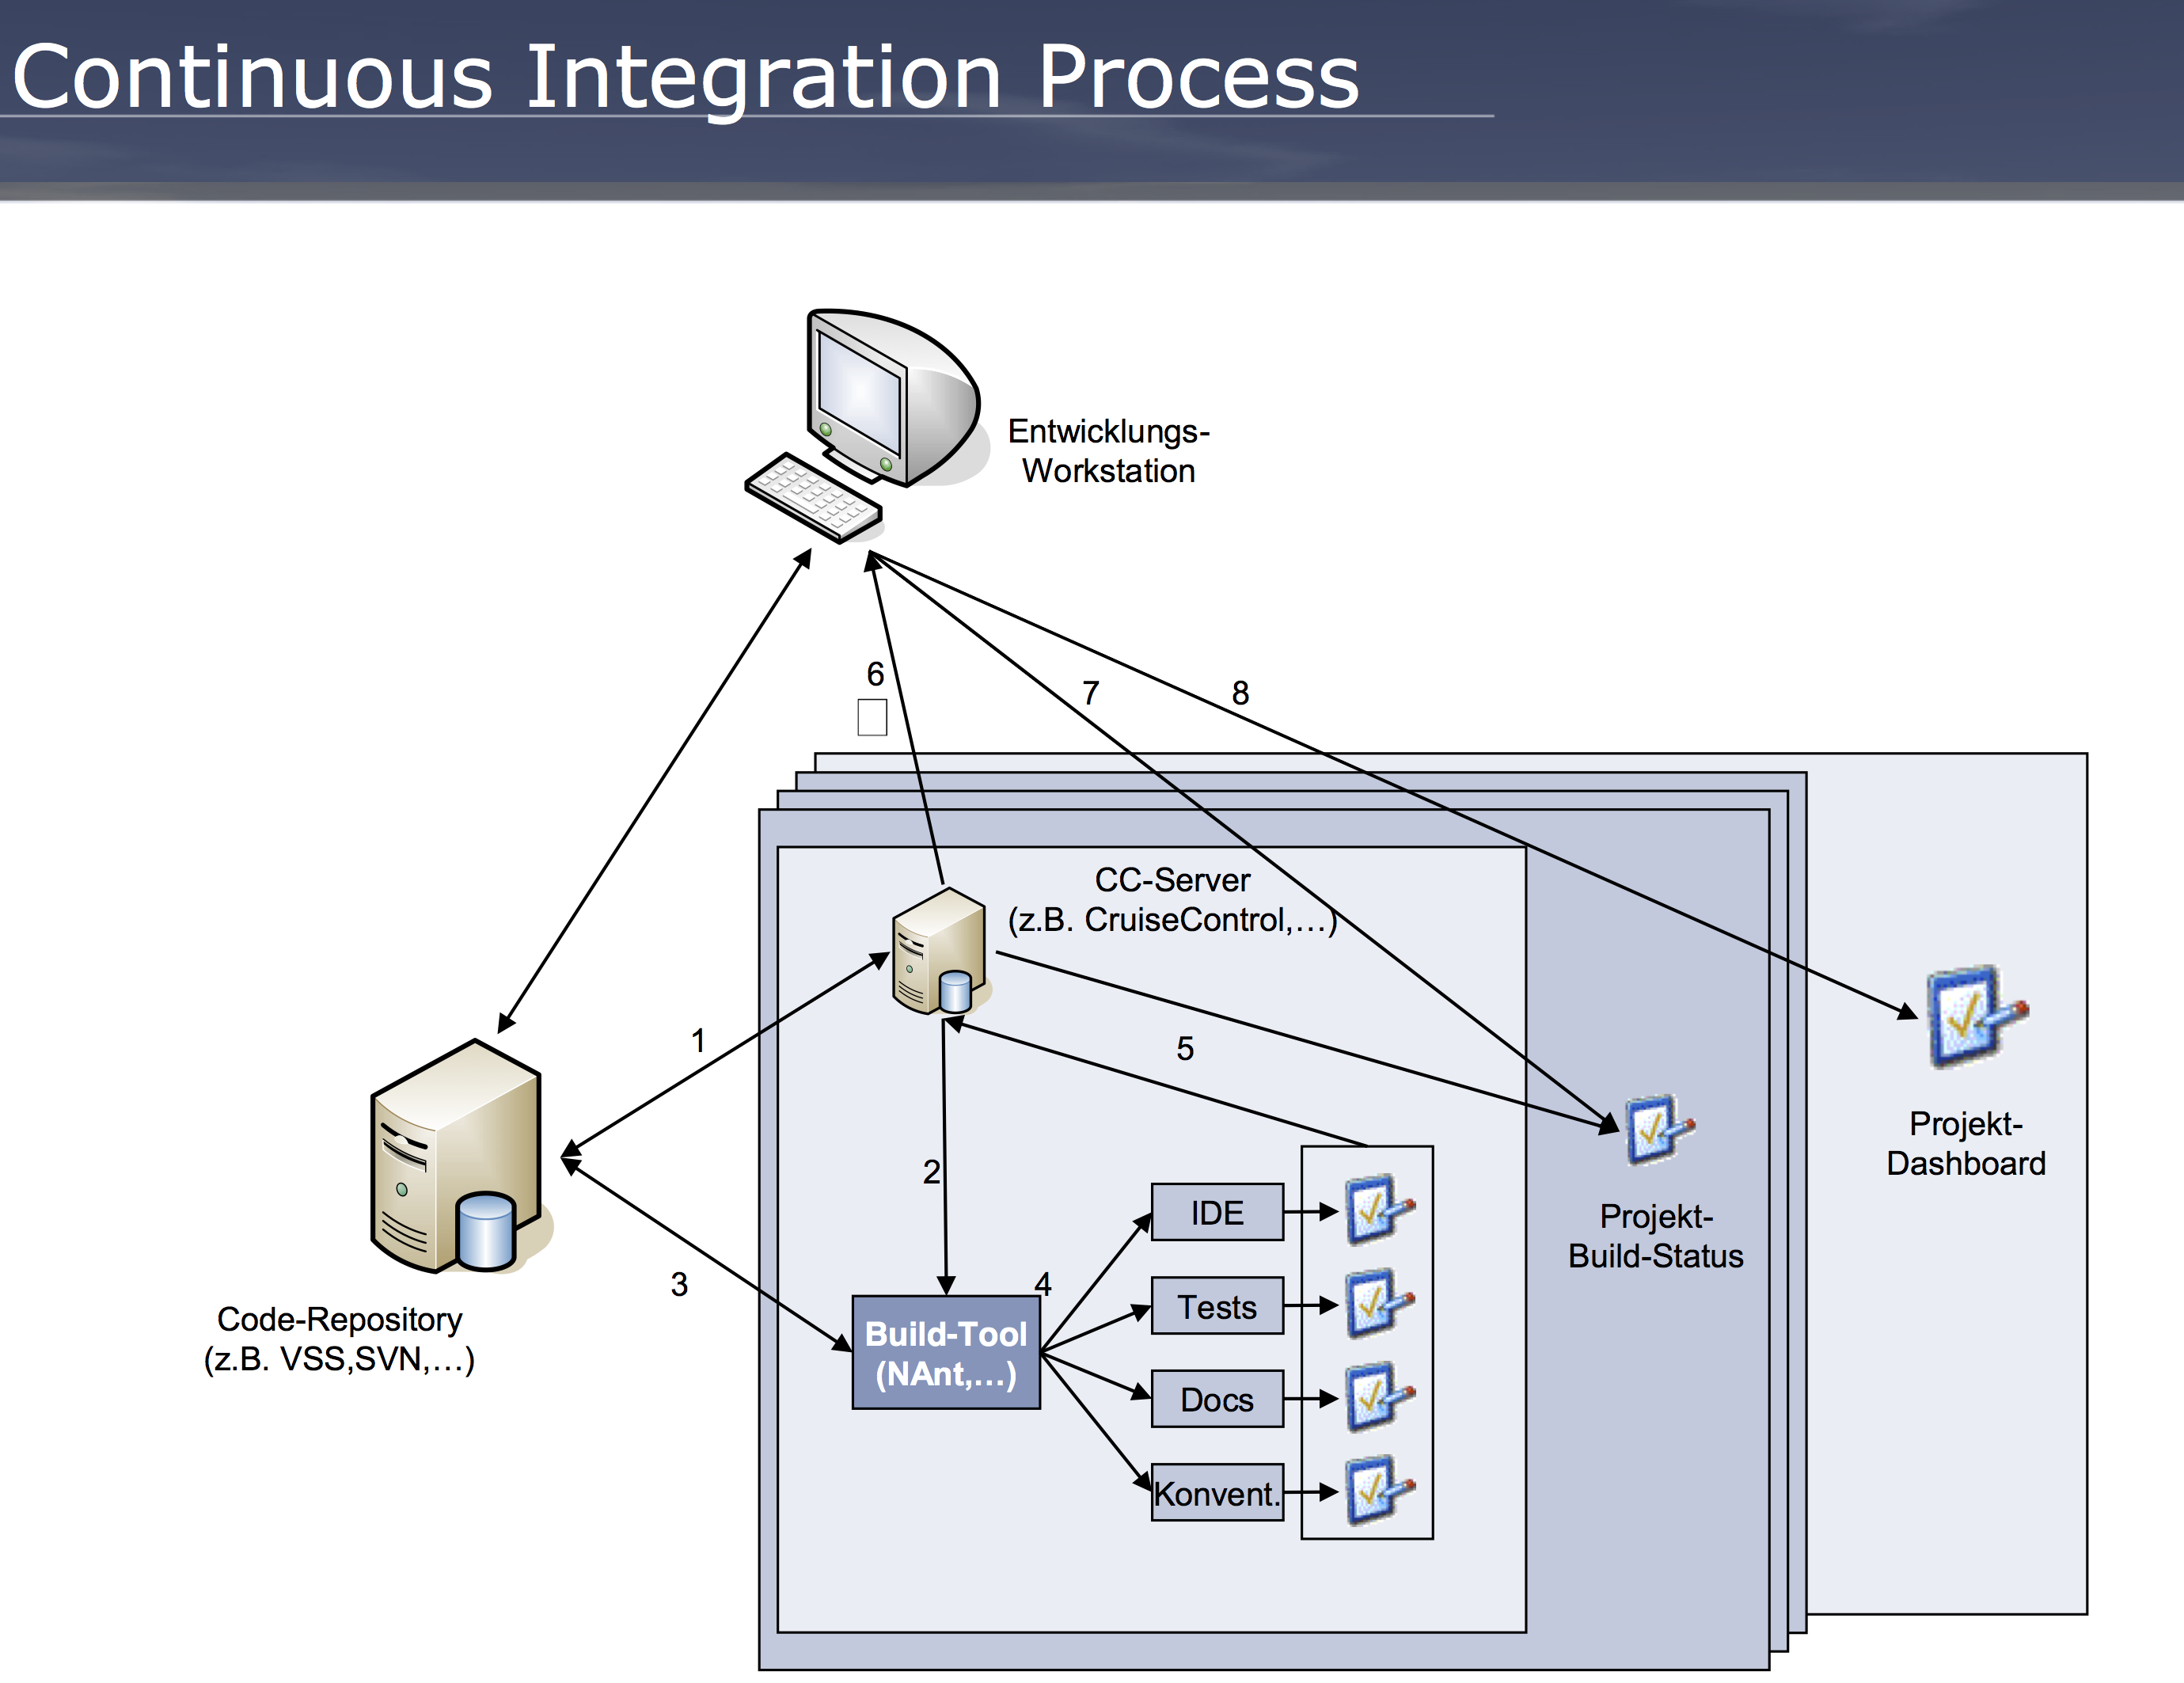
\includegraphics[width=0.8\textwidth]{img/continuousintegration.png}
	\caption{Continuous Build Prozess eines Softwareprojekts nach \cite{build-continuous}}
\label{fig:ci}
\end{figure}

\subsection{Die Kosten eines fehlgeschlagenen Builds}
Was passiert wenn der Build Prozess fehlschlägt, weil aus welchen Gründen auch immer die Abhängigkeiten nicht korrekt definiert wurden?
\\
Man unterscheidet hierbei bei den Fehlerentstehung zwischen einem \textit{Loud failure}, einem \textit{Silent failure} und einem \textit{Intentional failure}.
Der Loud failure ist ist der Zustand, wenn der Kompiler eine Datei nicht übersetzt, oder das Linking nicht korrekt ist und den Build zum Abbruch bringt.
Der Silent failure ist vermutlich ein schwer zu findenden Fehler, denn der Build war hier erfolgreich, aber der gewünschte Output ist nicht korrekt, weil \acs{z. B.} ein geänderter Code nicht re-kompiliert oder eine alte Bibliothek verwendet wurde.
\\
Der dritte Fehler, der Intentional failure, der vermutlich am  schwersten zu finden ist, entsteht, wenn der Quellcode Backdoors, \acs{etc.} enthält. \cite{software-analysis}

\subsection{Effektiver Build}
Wie kann man diesen Build Prozess denn nun verbessern, wenn oft etwas schief geht oder der Build Prozess sehr lange dauert?
\\
Folgende simple Antworten sind hierbei zu finden, \cite{software-analysis}:
\begin{itemize}
	\item Verbesserung der Qualität der Software
	\item Reduzierung von verschwendeter Zeit
	\item Verhinderung von Sicherheitsrisiken 
	\item Compliance Vorgaben einhalten 
\end{itemize}


\chapter{Versionsmanagement}

Moderne Softwareprogrammierung wird immer komplexer, sie muss meist von mehreren Programmierern gemeinsam erledigt werden, dies erfordert einen hohen Organisationsaufwand, da jeder Programmierer nur noch einen kleinen Teil des Quellcodes erstellt und diese Teile zusammengeführt werden müssen. Ferner besteht ein System sowohl aus verschiedenen Versionen als auch Varianten, dies muss ebenfalls gemanaged werden insbesondere um „Bugs“ zu verhindern.
\\
Das Erstellen einer neuen Version bedingt durch einen Ausschneiden, Einfügen oder Löschen von bereits vorhandenem Code wird dabei \Gu history step\Go (\cite{cm_vc}, S. 41) genannt. 
Die Schrittweise Entwicklung wird durch die Versionskontrolle nachvollziehbar gemacht, da sowohl das Original als auch die Vorgängerversion für jeden \Gu history step\Go erhalten bleiben. So ist die Entwicklung auch später noch nachvollziehbar und im Gegensatz zu einem herkömmlichen Back-Up wurde mit der Prämisse gearbeitet so viel Speicherplatz wie möglich zu sparen. Dies wird durch Kompressionsverfahren ermöglicht. \cite{cm_vc}
\\
Gemäß dem ITIL-Standard umfasst Versionsmanagement „alle Verfahren von der Anforderungsbearbeitung über die Planung der Umsetzung, Tests und Abnahme von Soft- und Hardwareversionen bis hin zur organisatorischen und technischen Vorbereitung der Einführung einer Komponente“. \cite{itil_infosec}, S. 20

\section{Anfänge der Versionierung}

\textbf{SCCS (Source Code Control System)}
\\
\acs{SCCS} wurde 1972 in den Bell Labs entwickelt und wurde später in C neu geschrieben um in UNIX Systemen eingesetzt werden zu können, diese Möglichkeit wurde auch genutzt weswegen SCCS in vielen UNIX-Distributionen zur Verfügung stand. Es war bis zum Erscheinen von RCS (siehe Unten) das am Meisten genutzte System zur Versionierung. 
\\
Die Idee von SCCS war, dass eine Software \Gu linear\Go entwickelt wird, also eine neuere Version seine jeweilige Vorgängerversion ablöst, wobei die Versionen dabei nach dem Schema \Gu X.Y\Go durchnummeriert werden. Bei einer größeren Änderung wird „X“ erhöht, bei einer kleineren Änderung das „Y“. Für jeden \Gu history step\Go wird dabei um Speicherplatz zu sparen nur das \Gu Delta \Go, also die Änderung im Vergleich zur Vorgängerversion, gespeichert. Die nachfolgende Abbildung verdeutlicht dies, die Quader stehen dabei für Versionen, die Dreiecke für die jeweiligen Deltas.
\begin{figure}[H]
	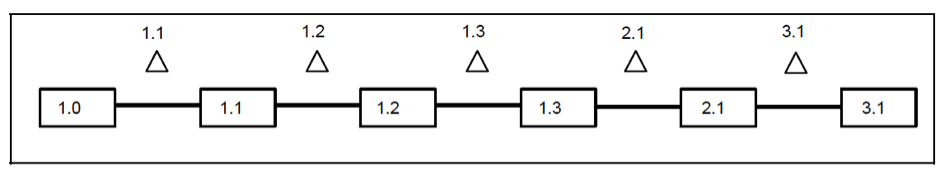
\includegraphics[width=\textwidth]{img/vcm1.png}
	\label{fig:vcm1}
	\caption{ SCCS nach \cite{cm_vc}, S. 43}
\end{figure}

Wichtig dabei ist, dass es sich um \Gu forward deltas \Go (\cite{cm_vc}, S. 43), also vorwärts gerichtete Deltas, handelt. Dies heißt, dass SCCS immer die Ursprungsversion speichert und für diese dann alle weiteren Änderungen. Die gesamte Speicherung erfolgt dabei in einer einzigen Datei und es ist auch möglich, dass eine Version zwei Nachfolger hat, jedoch nicht mehr als zwei. \cite{cm_vc}

\textbf{RCS (Revision Control System)}
\\
\acs{RCS} wurde in den 80ern als Alternative zu dem bis dahin sehr populären SCCS von Walter F. Tichy als freie Alternative zu diesem Veröffentlicht. Mit RCS wurden viele der Funktionen wie z.B. Speicherung, Logging oder das Zusammenführen von Codeteilen automatisiert und somit vereinfacht. RCS arbeitete damit hauptsächlich mit dem UNIX \textit{diff}-Kommando, das die Unterschiede zwischen zwei Dateien ermitteln kann.
\\
Wie auch \acs{SCCS} unterstützt \acs{RCS} jedoch nur eine einzelne Datei zur Speicherung des Codes und es fehlt auch die Unterstützung für komplette Projekte bzw. Ordnerstrukturen und es war Entwicklern auch nicht möglich gemeinsam an einem großen Projekt zu arbeiten.
\\
RCS war von Anfang an darauf ausgelegt, dass die Entwicklung einer Baumstruktur gleicht, also eine Version auch mehrere Nachfolgerversionen haben kann. Deswegen wird dies im Gegensatz zu SCCS auch besser unterstützt. Des Weiteren wurde in RCS auch das automatische Zusammenführen verschiedener Versionen implementiert. Dabei können Versionen von Verschiedenen Verästelungen automatisch zu einer neuen Version zusammengefasst werden und mögliche Differenzen in beiden Versionen werden Markiert und für den Programmierer sichtbar gemacht wodurch dieser manuell entscheiden kann welchen Teil des Codes er übernehmen will. Im Gegensatz zu SCCS wird in RCS auch nur die aktuellste Version gespeichert und alle anderen älteren \acs{bzw.} möglicherweise parallel erstellten Versionen sind über Deltas wiederherstellbar. Diese sind für denselben Ast rückwärts gerichtet und für eine Verästelung vorwärtsgerichtet. Ein Schema von RCS ist auf der nachfolgenden Abbildung ersichtlich. \cite{cm_vc}

\begin{figure}[H]
	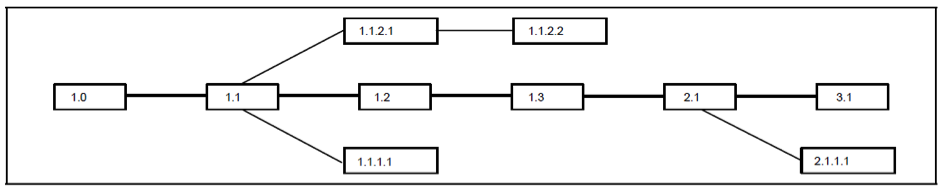
\includegraphics[width=\textwidth]{img/vcm2.png}
	\label{fig:vcm2}
	\caption {RCS nach \cite{cm_vc}, S.45}
\end{figure}

\textbf{Andere Versionierungssysteme}
\\
Natürlich sind die beiden erwähnten System (SCCS und RCS) nicht die einzigen verfügbaren Systeme. Es gibt weitere Möglichkeiten der Versionsverwaltung wie z.B. CVS oder VOODOO, auf diese soll jedoch nicht näher eingegangen werden. \cite{cm_vc}

\section{Anwendungsbeispiel - Git}
Ein verfügbares freies Programm für die Versionierung, welches heutzutage häufig genutzt wird, ist Git. Git wurde von Linus Torvalds ursprünglich für die koordinierte Entwicklung des Linux-Betriebssystems geschrieben. Im Gegensatz zu vielen anderen Tools arbeitet Git mit \Gu software revisions \Go (\cite{git_tool}, S. 1) und nicht mit Versionen die für viele Programmierer insbesondere bei Freizeitprojekten nicht von Belang sind. Stattdessen wollen diese nachvollziehen können welche Änderungen übernommen worden sind oder wie ein von ihnen geschriebener Code-Teil in das Programm eingebettet wurde.
\\
In Git werden die Dateien vergleichbar mit einem kleinen \Gu filesytem\Go (\cite{git_scm}, S.5) gespeichert, für jede Änderung wird ein Abbild der aktuellen Datenstruktur erzeugt, dies ist auf der  Abbildung \ref{fig:git} ersichtlich.
\\
Git ermöglicht es Programmierern das Komplette „Software-Repository“ zu kopieren und ihre eigenen privaten Zweige zu erstellen und zu löschen, kleine unvollständige Änderungen einzureichen oder die komplette Code-Revision zu vertagen. Ferner ermöglicht es Git den Programmierern genau festzustellen wo eine Änderung durchgeführt wurde und es behält einen kompletten Graph zur Übersicht über alle Änderungen, so müssen Sie sich nicht mit kleinen Dateien befassen in denen möglicherweise Änderungen erfolgt sind, sondern haben die Übersicht über das komplette Programm. 
\begin{figure}[H]
	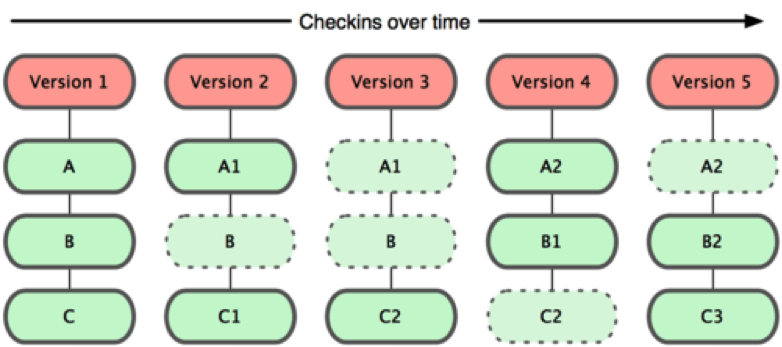
\includegraphics[width=0.9\textwidth]{img/git.png}
	\caption{Git nach \cite{git_scm}, S.5}
	\label{fig:git}
\end{figure}

Die private Kopie des Repositorys ermöglicht auch neue Arbeitsabläufe. So können Programmierer z.B. gegenseitig den Code von ihren Repositorys laden oder ein Integrations-Manager kann von jedem seiner Programmierer frei und ohne diese zu beeinflussen Code holen und diesen in das „master repository“ (\cite{git_tool}, S2) einbetten. Ferner ermöglicht es Programmierer zu entlasten, da das Coding mehrstufig aufgebaut werden kann. Dies heißt, dass vergleichbar mit der Linux-Kernel-Entwicklung zunächst die Programmierer den Code schreiben, in der nächsten Stufe wird dieser Code in Teilprojekte integriert welche dann wiederum in das Gesamt-Projekt integriert werden können.
\\
Ein weiterer Vorteil der lokalen Speicherung besteht darin, dass ein Programmierer nicht zwangsläufig Zugang zum Internet benötigt. Stattdessen kann er seine Änderungen „offline“ implementieren und zu einem Zeitpunkt seiner Wahl zum „master repository“  hinzufügen. Des Weiteren sind die Zugriffszeiten bei dieser Art der Speicherung geringer und die Produktivität sollte steigen.
\\
Git ermöglicht es zudem ein Repository für die Öffentlichkeit zur Verfügung zu stellen. Mittlerweile kann dieses auch von einem Drittanbieter wie etwa GitHub gehostet werden. Wobei der Anbieter das „repository management“ (\cite{git_tool}, S. 2) über eine Browser-Schnittstelle gewährleistet. 
\\
\cite{git_scm}, \cite{git_tool}


\chapter{Release Management}
\section{Aufgaben und funktionale Einordnung}
Das Release Management ist für die effektive, sichere und nachvollziehbare Durchführung von Änderungen der IT-Infrastruktur verantwortlich. Aufgaben des Release Managements sind die Planung, Überwachung und Durchführung von Rollouts und Rollins. Dies erfolgt in Abstimmung mit dem Change Management.  Ferner hat das Release Management die Aufgabe die Gesamtheit der Änderungen der IT zeitlich, technisch und inhaltlich zu bündeln und aufeinander abzustimmen. \cite{wiki-it}, \cite{rm-pilorget}
\\
Die Funktion des Release Management ist dem Service Support zugeordnet. Dieser hat die operativen Prozesse zur Behandlung von Service-Unterbrechungen und Durchführung zur Aufgabe und garantiert somit die Aufrechterhaltung der IT-Services. Der Service Support ist wiederum dem IT Service Management zugeordnet.  \cite{wiki-it-service}

\section{Einteilung von Releases}
\textbf{Emergency Release:}
\\
Behebung von Störungen oder signifikanten Problemen in der IT. Ähnelt dem Minor Release, benötigt jedoch \acs{i. d. R.} viel weniger Zeit.
\\
\textbf{Minor Release:}
\\
Dieser Release enthält kleinere Erweiterungen und Fixes. Werden häufiger als Major Releases durchgeführt, benötigen jedoch weniger Zeit und Planung. Ersetzen voran-gegangene Emergency Releases. 
\\
\textbf{Major Release:}
\\
Beinhaltet signifikante neue Funktionalitäten, Upgrades, oder neue Services in der IT. Ersetzen alle vorangegangen Minor und Emergency Releases, welche bezüglich eines Problems in der IT durchgeführt wurden und macht diese überflüssig. Dieser Release wird selten durchgeführt, benötigt jedoch mehr Zeit und Planung als Minor und Emergency Releases.
\cite{rm-howard}
\section{Teilprozesse}
Die Teilprozesse des Release Management nach ITIL sind in der folgenden Abbildung \ref{fig:tp} dargestellt. 
\begin{figure}[H]
	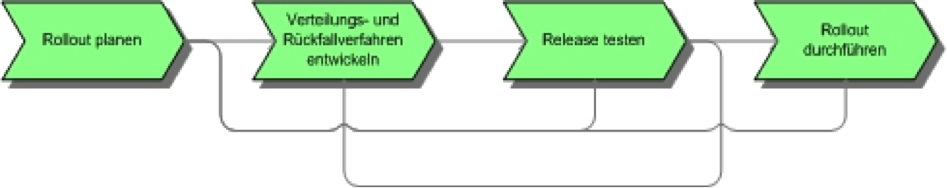
\includegraphics[width=\textwidth]{img/Teilprozesse.png}
	\caption{Teilprozesse des Release Management nach ITIL \cite{wiki-it}}
	\label{fig:tp}
\end{figure}
\textbf{Rollout planen:}
\\
Für die Planung eines Release wird eine Vielzahl von Informationen benötigt. Diese sind in einem Release-Plan und einem Release-Steckbrief gebündelt. \cite{rm-schiefer-erik}
\\
\textbf{Release-Plan:}
\begin{itemize}
	\item Abstimmung über den Inhalt des Releases
	\item Absprache über zeitliche Reihenfolge, Standorte und Organisationsbereiche
	\item Klärung der eingesetzten Hard- und Software
	\item Klärung der erforderlichen Mittel für Hardware, Software und Dienstleistungen
	\item Abstimmung der Verantwortlichen
	\item Dienstleistungen, welche von Dritten benötigt und über das Supplier Management koordiniert werden
	\item Erstellen von Back-Out-Plänen
	\item Aufwandsabschätzung
\end{itemize}
\textbf{Release-Steckbrief:}
\begin{itemize}
	\item Name des Release
	\item Version des Release
	\item Beschreibung des Release
	\item Dokumentationsablage
	\item Historie
\end{itemize}


\textbf{Verteilungs- und Rückfallverfahren entwickeln:}
\\
In diesem Teilprozess werden die technischen Voraussetzungen zur Installation, bzw. der Verteilung der neuen Komponenten des Release geschaffen. Des Weiteren werden hier Vorkehrungen für das Zurückfahren des Rollouts für den Fall von unvorhergesehenen Problemen getroffen. \cite{wiki-it}
\\
\textbf{Release testen:}
\\
Der Test des Release erfolgt in der Regel durch das Betriebspersonal (=> Realitätsnähe). Besonderer Beachtung sollten hierbei der Funktionsweise, den technischen Betriebs-aspekten, dem Leistungsverhalten und der Integration in die vorhandene Infrastruktur geschenkt werden.  
\cite{rm-schiefer-erik}
\\
Im Rahmen des Release Prozesses sind drei Arten von Tests vorgesehen. Dies sind der Unit-, Integration- und der Abnahme-Test. \cite{rm-pilorget} 
\\
Für den Unit-Test ist der Applikationsexperte verantwortlich. Hierbei wird geprüft, ob jedes Element des Release so funktioniert, wie es spezifiziert wurde. Es werden Testprogramme und Testskripte geschrieben. Hierbei werden einfache Testfälle benutzt. 
Die Verantwortung für den Integration Test trägt der IT-Projektleiter. Dieser überprüft, ob die definierten Funktionen und Schnittstellen funktionieren und im Verbund funktionieren. Hierbei sollen möglichst alle Benutzer-Szenarien berücksichtigt werden. 
Für den Abnahme-Test ist der Fachprojektleiter verantwortlich. Dieser Test unterteilt sich in einen User Acceptance Test und einen Regression Test. Im User Acceptance Test wird geprüft, ob das System alle geforderten Business-Funktionalitäten abdeckt und den korrekten Output generiert. Im Regression Test wird sichergestellt, dass die System-veränderungen nicht einen vorher funktionierenden Systemteil beeinflusst haben. 
\\
\textbf{Rollout durchführen:}
\\
Dieser Prozess hat einerseits zum Ziel, die Release-Komponenten in die IT-Umgebung auszurollen. D.h. die neuen Funktionalitäten werden auf alle Zielobjekte ausgebreitet und installiert. Die Mitarbeiter, welche von den Änderungen der Releases betroffen sind, werden geschult. Die Dokumentation über entsprechende Konfigurationselemente wird aktualisiert. 
\cite{rm-pilorget}
\\ 
Andererseits findet eine Erfolgskontrolle statt. \cite{wiki-it}


\chapter{Change Management}



\chapter{Fazit}
Lorem ipsum dolet.


%Ende / Verzeichnisse
\appendix
\renewcommand{\chaptermark}[1]{%
\markboth{ #1}{}}

\chapter{Anhang}
Im Sinne dieses Seminar wurde die Ausarbeitung mit LaTex in Git erstellt.
Das Projekt ist unter folgender Adresse zu finden.
\\
\url{https://github.com/dgbass/Seminar_EBIS}



\backmatter

%\thispagestyle{empty}
\chapter{Abkürzungsverzeichnis}
%\thispagestyle{empty}
%\pagenumbering{roman}

\begin{acronym} [-------------]
\acro{AWS}{Amazon Web Service}
\acro{BI}{Business Intelligence}
\acro{BW}{Business Warehouse}
\acro{bzw.}{beziehungsweise}
\acro{CPU}{Central Processing Unit}
\acro{CSV}{Comma-separated Values}
\acro{d.h.}{das heißt}
\acro{DOC}{Dokumente (in Word)}
\acro{ECDA}{Enterprise Connect Data Access}
\acro{ERP}{Enterprise-Resource-Planning}
\acro{ETL}{Extraktion, Transformation, Laden}
\acro{etc.}{et cetera}
\acro{FOX}{Formula eXtension}	
\acro{ggf.}{gegebenenfalls}
\acro{HANA}{High Performance Analytics Appliance}
\acro{HDD}{Hard Disk Drive}
\acro{HTML}{Hypertext Markup Language}
\acro{IMDB}{In-Memory Database}
\acro{I/O} {Input/Output}
\acro{i. d. R.}{in der Regel}
\acro{IP}{Internet Protocol}
\acro{ISO}{Internationale Organisation für Normierung}
\acro{JDBC}{Java Database Connectivity}
\acro{MDX}{Multidimensional Expressions}
\acro{MMDB}{Main Memory Database}
\acro{MVCC}{Multiversion Concurrency Control}
\acro{NVRAM}{Non-volatile Random-Access Memory}
\acro{ODBC}{Open Database Connectivity}
\acro{ODP}{Operational Data Provider}
\acro{OLAP}{Online Analytical Processing}
\acro{PAL}{Predictive Analysis Library}
\acro{PC}{Personal Computer}
\acro{PDF}{Portable Document File}
\acro{RAM}{Random-Access Memory}
\acro{RCP}{Rich-Client Platform}
\acro{RCS}{Revision Control System}
\acro{RDBMS}{relationale Datenbankmanagementsysteme}
\acro{SAP}{SAP AG}
\acro{SCCS}{Source Code Control System}
\acro{SCM}{Software Configuration Management}
\acro{SLT}{SAP Landscape Transformation}
\acro{SQL}{Structured Query Language}
\acro{TCP}{Transmission Control Protocol}
\acro{URL}{Uniform Ressource Locator}
\acro{VCS}{Version Control System}
\acro{XLS}{Excel Spreadsheet}
\acro{XLSX}{Excel Spreadsheet}
\acro{XML}{Extensible Markup Language}
\acro{z. B.} {zum Beispiel}


\end{acronym}


%\newpage \vspace*{2cm} \pagestyle{empty}


%Einbinden des Abbildungsverzeichnisses
\listoffigures

%Einbinden des Literaturverzeichnisses
\bibliography{bibliography}


\end {document}

% Local Variables:
% eval: (longlines-mode 1)
% TeX-engine: default
% End:
